\documentclass[conference]{IEEEtran}
\IEEEoverridecommandlockouts
\usepackage{cite}
\usepackage{amsmath,amssymb}
\usepackage{graphicx}
\usepackage{booktabs}
\usepackage{url}
\usepackage[hidelinks]{hyperref}
\usepackage{microtype}
% Generated by paper/make_tables.py -- do not edit.
\newcommand{\nTasks}{321}
\newcommand{\nPairs}{45}
\newcommand{\nSeeds}{5}
\newcommand{\nGrades}{8,025}
\newcommand{\bootReplicates}{4,000}
\newcommand{\bootUnits}{276}
\newcommand{\planExact}{91.9}
\newcommand{\planGap}{28.63}
\newcommand{\planGapCI}{28.63 [14.22, 44.96]}
\newcommand{\gateExact}{85.4}
\newcommand{\gateGap}{31.37}
\newcommand{\gateGapCI}{31.37 [16.41, 48.27]}
\newcommand{\vsGateGap}{-2.74 [-3.80, -1.80]}
\newcommand{\vsGateExact}{6.5 [4.1, 9.2]}
\newcommand{\planPassK}{91.9 [89.8, 94.1]}
\newcommand{\gatePassK}{85.4 [81.6, 89.4]}
\newcommand{\reactPassK}{17.4 [13.9, 20.7]}
\newcommand{\costSettings}{27}
\newcommand{\costPlannerBetter}{27}
\newcommand{\ablShield}{0.00 [0.00, 0.00]}
\newcommand{\ablVoi}{0.00 [0.00, 0.00]}
\newcommand{\ablPrior}{11.45 [4.81, 19.18]}
\newcommand{\ablRule}{18.30 [9.49, 29.93]}
\newcommand{\settleMarginal}{0.72}
\newcommand{\settleLate}{0.50}
\newcommand{\optPrem}{66.0}
\newcommand{\optShieldPrem}{7.0}
\newcommand{\optPaired}{253.53}
\newcommand{\optShieldPaired}{192.20}
\newcommand{\optShieldGap}{244.29}
\newcommand{\optGap}{163.61}
\newcommand{\transferHidden}{-2.67 [-3.67, -1.75]}
\newcommand{\wrongPrior}{201.22}


\begin{document}

\title{Deciding Under Uncertain Payment Finality:\\A Decision Rule That Prices Its Options}

\author{\IEEEauthorblockN{Abhishek Sharma}
\IEEEauthorblockA{Senior Member, IEEE\\
\texttt{abhicse24@gmail.com} \quad ORCID: 0009-0007-1103-2103}}

\maketitle

\begin{abstract}
When a merchant's payment capture will not resolve before the order's ship-by
date, an agent has to choose without knowing. FinalityBench's strongest policy
escalates to a human, which is safe and, on that corpus, never the best
available action: escalation costs a flat fee on every case while the
alternatives cost something that depends on the order.

We replace the fixed rule with an expected-value comparison under a belief
fitted from the benchmark's public split. It is a deadline decision rule, not a
general sequential planner: a conditional probability and one comparison of
four closed-form expressions, with no search over action sequences. Over
\nTasks{} tasks under \nSeeds{} fault schedules --- \nRuleEpisodes{} episodes
of the rule, \nGrades{} across all \nPolicies{} policies --- it is exactly
correct on \planExact\%\ against the gate's \gateExact\%,
and on a paired resample it reduces the mean position gap by
\$\vsGateReduction{} per episode.

The margin turns on what escalation is worth, not only on what it costs.
FinalityBench's analyst starts no new money movement, so escalation cannot
rescue a capture that never settles. Re-scoring every episode under more
capable analysts shrinks the gap from \$\escBaselineGap{} to \$\escFullGap{}
without changing its sign: only \escRescuable{} of the gate's
\escEscalations{} escalations are on cases a retry could rescue. A sweep over
\costSettings{} cost settings reuses the same tasks and seeds, so it varies one
experiment rather than confirming the result \costSettings{} times.

Two of four components contribute nothing. The safety shield is inert because
the decision rule already maximises expected value, and pursuing why gave the
more transferable result: an expected-value shield cannot object to shipping
without checking, because at this settle rate that bet pays, while a shield
reasoning about the branch it cannot rule out cuts a ship-on-first-sign
policy's pre-determination irreversible actions from \optPrem\%\ to
\optShieldPrem\%\ and is worse on the corpus's own outcome distribution.
\end{abstract}

\begin{IEEEkeywords}
planning under partial observability, value of information, safety shields,
irreversible actions, payment systems, risk-sensitive decision making
\end{IEEEkeywords}

\section{Introduction}

A capture was submitted eight minutes ago. The order ships today or the customer
cancels. The processor's authoritative endpoint says the outcome is not yet
determined, and it is telling the truth: the outcome has not happened. In four
hours it will, and by then the order is gone.

What should the agent do?

FinalityBench~\cite{finalitybench} poses this and grades the answer in money.
Its strongest policy gates every irreversible action on an authoritative probe
and, when the probe still says unknown at the deadline, hands the case to a
human. That policy is exactly right about the mechanism, and it reaches
\gateExact\%\ exactly correct across the benchmark. Its remaining loss is almost
entirely on one archetype: the cases whose outcome lands after the ship-by date,
where it escalates every time.

Escalation is a decision, and it has a price. So do the alternatives. Closing
the case costs a dispute fee whenever money later arrives for an order that was
never fulfilled, which happens with probability equal to the chance the capture
settles. Shipping collects the order when the capture settles and loses the cost
of goods when it does not. Which is cheapest depends on the order value, and no
fixed rule can track that.

This paper replaces the fixed rule with a valuation. The valuation is a
deterministic computation at a single instant, the deadline, and not a search
over action sequences. The contributions:

\begin{itemize}
\item \textbf{A belief over finality fitted from data}, in which an
authoritative probe returning unknown is treated as the evidence it is: it rules
out every resolution time up to now, and the settle rate must be conditioned on
that rather than taken from the margin (Section~\ref{sec:belief}).

\item \textbf{An expected-value decision at the deadline}, which reproduces the
gate's behaviour everywhere the gate is right and departs from it only where
escalation is not the best-priced option (Section~\ref{sec:planner}).

\item \textbf{Evidence that the departure is worth something}:
\$\vsGateReduction{} less per episode on a shared task resample, holding across
\costPlannerBetter{} of
\costSettings{} cost settings and on a corpus the belief was not fitted to
(Section~\ref{sec:results}).

\item \textbf{A negative result about safety shields.} Inside a planner that
already maximises expected value, a shield is inert, and we report the
\$\ablShield{} it is worth. Around a policy that gambles, the criterion matters:
an expected-value shield permits the gamble because the gamble pays, and only a
downside criterion refuses it (Section~\ref{sec:shield}).
\end{itemize}

\section{Related work}

\textbf{Knowing when not to act.} Luo et al.~\cite{abstention} treat abstention
as a sequential decision in which an agent may answer, abstain, or gather more
information at each turn, and find agents struggle when a task looks feasible
until the environment says otherwise. That is the shape of the problem here.
The difference is that abstention in their setting is a free action, while
escalation here has a price that competes with the alternatives, and it is the
competition that this paper is about. DosSantos DiSorbo and
Ju~\cite{actorescalate} do price it: their agent predicts, estimates its own
chance of being right, and weighs the expected cost of acting against the cost
of handing the case to a human. They find that language models carry
model-specific escalation profiles and that miscalibrated ones act when they
should defer and defer when they should act. That is a question about the
agent; this paper asks the prior question of what the correctly priced answer
is, computes it rather than learning it, and finds that the benchmark's fixed
escalation rule is the thing that is miscalibrated.

\textbf{Shields and runtime enforcement.} ShieldAgent~\cite{shieldagent}
enforces safety policies over an agent's action trajectory by extracting
verifiable rules from policy documents and checking compliance. That is a
rule-based criterion: an action is blocked because it violates a stated policy.
The shield here is a value criterion, blocking an action because the branch the
agent cannot rule out is worse than the best reversible alternative. The two are
complementary and answer different questions, and Section~\ref{sec:shield}
suggests the value criterion is the weaker of the two on its own.

\textbf{Value of information.} Laouar et al.~\cite{voimcp} exploit the fact that
the value of information varies across the belief space, skipping observation
branches in Monte Carlo tree search where it is low. Feng et
al.~\cite{coststopping} make a related argument for tool acquisition, proving
that score-only rules are suboptimal when tools cost different amounts. Our
probing rule is the same idea at a much smaller scale, and
Section~\ref{sec:results} reports that at this scale it buys nothing.

\textbf{Verified tool calls.} The baseline we measure against implements
postcondition checks, keyed retries and verify-before-retry as recommended by
Mansoor et al.~\cite{verifiedtools}, plus the finality gate the benchmark adds.
It is a strong baseline rather than a straw one, and the margin over it is
correspondingly small.

\textbf{Accounting after the agent stops.} Nandi et
al.~\cite{trustbound} ask what a payment service can still guarantee once an
agent has stopped while its operations remain executable. Their Lean
development proves that an admission fence fixes a journal covering every
effect and outstanding right, and that discharging those rights prevents
further effects: completeness of the account, and termination of payment
authority. That is the complementary half of the problem. They make the
reckoning exact once the outcomes are known; the decision priced here is taken
while the outcome does not yet exist and no fence can bring it forward.

\textbf{Reversibility.} Zhai et al.~\cite{revisable} classify actions by whether
they can be undone and show that an agent's flexibility is bounded by its
reversibility. The valuation here is one way of pricing that bound.

\section{Setting}

A FinalityBench episode is one order with one pending capture. Four systems hold
partial and conflicting views, an authoritative probe returns a terminal status
only once the outcome exists, and every tool costs simulated time against a
ship-by deadline. Grading is on the merchant's terminal economic position,
reported as the gap to a privileged reference that is told when the capture
resolves.

We reuse the released artifact rather than reimplementing it, and every result
records the revision it ran against. The corpus is \nTasks{} tasks including
\nPairs{} twin pairs, whose two members are indistinguishable at the decision
instant and whose eventual correct dispositions differ.

Every policy is run on every task under \nSeeds{} fault schedules, so each
contributes \nTasks{} $\times$ \nSeeds{} $=$ \nRuleEpisodes{} episodes and the
\nPolicies{} policies compared give \nGrades{} graded episodes in total. A rate
reported for a single policy, the exact rate included, is over that policy's own
\nRuleEpisodes{}, not over the \nGrades{}.

\section{A belief about finality}
\label{sec:belief}

The only latent fact that matters is when the capture resolves and which way.
A probe that returns unknown at time $t$ rules out every resolution time up to
$t$, so the belief is the prior truncated by the latest unknown probe.

The prior is estimated from the benchmark's public split. One detail in it
carries most of the paper's remaining margin. The overall rate at which captures
settle on this corpus is \settleMarginal. The rate among captures that have not
resolved by the ship-by deadline is \settleLate. Captures that resolve late are
not a random sample of captures, and a planner that uses the marginal figure
concludes that shipping is profitable on exactly the cases where it is a coin
flip. The ablation in Section~\ref{sec:results} prices that mistake at
\$\ablPrior.

\section{Pricing the options}
\label{sec:planner}

At the deadline, with the outcome still unknown and a settle probability $p$,
an order worth $A$ with cost of goods $c$, dispute fee $D$ and escalation cost
$E$:

\begin{align}
V_{\text{ship}}     &= pA - c \\
V_{\text{close}}    &= -pD \\
V_{\text{escalate}} &= -E - D \Pr[\text{settles after the analyst looks}] \\
V_{\text{refund}}   &= -(1-p)A
\end{align}

Shipping collects the order when the capture settles and loses the goods when it
does not. Closing costs a dispute whenever money arrives for an order that was
never fulfilled. Escalation pays a flat fee for an analyst who returns the money
if it has arrived by the time they look, and still incurs the dispute when it
arrives afterwards. Refunding returns money that may never have come, which is
why it is almost always worst and is included so the comparison is complete.

At the benchmark's stipulated costs and $p$ near a half, escalation is never the
maximum. Below roughly \$125 of order value the gamble is cheap enough to take;
above it, closing bounds the loss at half the dispute fee. The planner computes
this rather than being told it, which is why Section~\ref{sec:results} can move
the constants and watch the decision follow.

\begin{figure}[t]
\small
\hrule\vspace{2pt}
\textbf{Planner}\; (case, deadline $T$)
\vspace{2pt}\hrule\vspace{3pt}
\begin{tabbing}
xx\=xx\=xx\=\kill
1\> \textbf{loop} \\
2\> \> $s \gets$ probe($\mathit{ref}$) \textbf{if} worth probing \textbf{else} last status \\
3\> \> \textbf{if} $s =$ settled \textbf{then return} ship \\
4\> \> \textbf{if} $s =$ failed \textbf{then} \\
5\> \> \> resubmit under the original key; \textbf{verify}; ship or close \\
6\> \> \textbf{if} $T - t > \delta$ \textbf{then} wait($\delta$); \textbf{continue} \\
7\> \> $p \gets \Pr[\text{settles} \mid \text{unresolved at } t]$ \\
8\> \> \textbf{return} $\arg\max \{V_{\text{ship}}, V_{\text{close}},
        V_{\text{escalate}}, V_{\text{refund}}\}$
\end{tabbing}
\vspace{-4pt}\hrule
\caption{The planner. Lines 1--6 are the finality gate's behaviour. Line 7
conditions on what the probes have ruled out, and line 8 is the departure: the
gate escalates unconditionally where this prices the options.}
\label{fig:algorithm}
\end{figure}

Everything else the planner does matches the gate: probe, wait while the
deadline allows, retry a failed capture under the original key, and verify the
replacement before shipping it. The last of those is not incidental. An earlier
version shipped as soon as a replacement was submitted, which gives away the
cost of goods whenever the replacement does not settle. Reconstructing that
version and running both costs \$\prematureCost{} per case on
\texttt{\prematureArchetype}, and takes exact resolution from
\prematureExactAfter\%\ to \prematureExactBefore\%.

It is worth saying what does \emph{not} happen. FinalityBench's premature flag
does not move at all, because it fires when an agent ships while the
\emph{original} capture reference is undetermined, and on this archetype the
original has already failed by the time a replacement exists. Shipping against
an unsettled replacement is the same mistake against a different reference and
the flag cannot see it, so the cost shows up in excess loss alone. An earlier
draft of this paragraph called it the premature action the benchmark detects,
which it is not.

\section{Results}
\label{sec:results}

\begin{table*}[t]
\centering
\caption{Policies over \nTasks{} tasks and \nSeeds{} seeds. Brackets are 95\%
bootstrap intervals over \bootUnits{} independent units, twin pairs resampled
together.}
\label{tab:main}
\footnotesize\setlength{\tabcolsep}{6pt}
\begin{tabular}{lrrrr}
\toprule
policy & exact (\%) & mean gap (\$) & paired (\$) & pre-det.\ (\%) \\
\midrule
rule-based SOP & 34.0 [29.8, 38.1] & 204.54 [173.09, 236.57] & 146.69 & 0.0 \\
reflection & 53.5 [49.0, 58.1] & 129.61 [106.96, 154.63] & 116.97 & 0.0 \\
ReAct loop & 54.0 [49.5, 58.5] & 128.19 [105.94, 152.40] & 116.97 & 0.0 \\
finality gate & 85.4 [79.9, 90.2] & 31.37 [16.41, 48.27] & 103.91 & 0.0 \\
\bfseries planner (this paper) & 91.9 [89.0, 94.6] & 28.63 [14.22, 44.96] & 95.54 & 2.5 \\
\bottomrule
\end{tabular}
\end{table*}

\begin{table}[t]
\centering
\caption{Differences on a shared task resample. Both policies face identical
tasks, so the comparison should use that rather than compare two marginal
intervals that overlap.}
\label{tab:paired}
\footnotesize\setlength{\tabcolsep}{3pt}
\begin{tabular}{lrr}
\toprule
comparison & mean gap (\$) & exact rate (pp) \\
\midrule
planner $-$ rule-based SOP & -175.91 [-206.61, -145.13] & 57.9 [54.1, 61.8] \\
planner $-$ reflection & -100.98 [-123.33, -81.62] & 38.4 [35.0, 41.7] \\
planner $-$ ReAct loop & -99.55 [-120.91, -80.65] & 37.9 [34.7, 41.3] \\
planner $-$ finality gate & -2.74 [-3.80, -1.80] & 6.5 [4.1, 9.2] \\
\bottomrule
\end{tabular}
\end{table}

\begin{figure}[t]
\centering
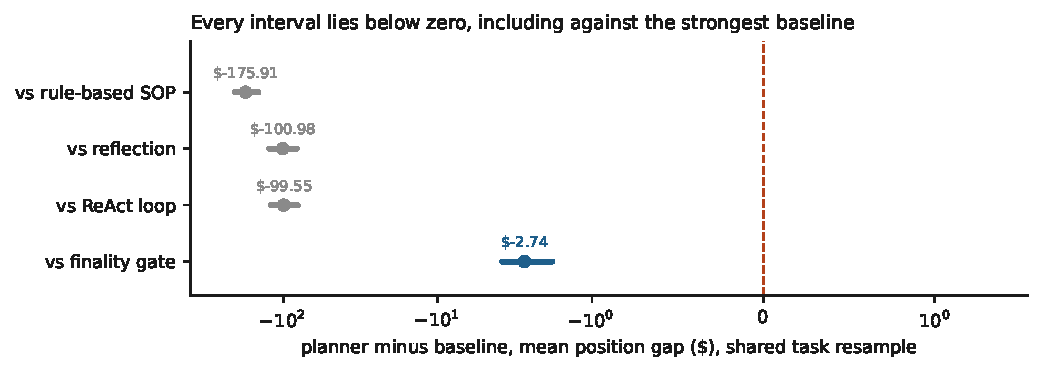
\includegraphics[width=\columnwidth]{../figures/fig1_comparison.pdf}
\caption{Planner minus baseline, mean position gap. Every interval lies below
zero, including against the strongest baseline, where the margin is small.}
\label{fig:comparison}
\end{figure}

\subsection{Against the baselines}

Table~\ref{tab:main} gives the marginal numbers and Table~\ref{tab:paired} the
comparisons. The planner reaches \planExact\%\ exact against the gate's
\gateExact\%. Its marginal interval, \$\planGapCI, overlaps the gate's
\$\gateGapCI{} almost entirely, which is why the marginal numbers are not the
evidence. On a resample that gives both policies the same tasks, the rule
reduces the mean gap by \$\vsGateReduction{} and raises the exact rate by
\vsGateExact{} points, and neither interval contains zero. Throughout, a
paired contrast is reported as the magnitude of the rule's improvement with
its interval in the same direction; the underlying signed difference is
\$\vsGateGap{}.

The margin over the gate is small in absolute terms and it should be read that
way. Against the weaker baselines it is two orders of magnitude larger, which
says more about those baselines than about this planner.

\subsection{One case, end to end}

Take an order of \$\exBigAmount{} whose capture resolves at $t=720$, past a ship-by
deadline of $t=600$. Both policies probe at intervals and both learn nothing,
because there is nothing yet to learn.

At $t=545$ the gate has about a minute of deadline left, no terminal status,
and a rule that says escalate. It escalates. An analyst picks the case up two
hundred ticks after the deadline, finds the money has arrived for an order that
can no longer ship, and returns it. The merchant is out the \$\exEscalate{}
handling cost.

The planner reaches the same instant with the same information and computes
four numbers. Shipping is worth $0.5 \times \exBigAmount{} - \exBigCogs{} =
-\$\exBigShip{}$, since the goods can still go out but the capture is a coin
flip. Closing is worth $-\$\exBigClose{}$, the dispute that follows when money
arrives for an unfulfilled order. Escalating is worth $-\$\exEscalate{}$ plus
the dispute it does not avoid. Refunding is worth $-\$\exBigRefund{}$, since
half the time there is nothing to refund. It closes, and saves
\$\exBigSaved{}.

On a \$\exSmallAmount{} order the same computation gives a different answer:
shipping is worth $-\$\exSmallShip{}$ against closing's $-\$\exSmallClose{}$, so
it ships and accepts the risk. The gate escalates in both cases for
\$\exEscalate{}.

\subsection{Where the margin comes from}

\begin{table}[t]
\centering
\caption{The planner against the gate, by archetype. The margin is concentrated
where the gate escalates.}
\label{tab:archetype}
\footnotesize\setlength{\tabcolsep}{4pt}
\begin{tabular}{lrrr}
\toprule
archetype & gate (\$) & planner (\$) & difference (\$) \\
\midrule
unresolvable & 245.16 & 226.28 & -18.88 \\
pending fail & 15.96 & 13.16 & -2.80 \\
pending fail hard & 1.38 & 0.00 & -1.38 \\
late chargeback & 0.00 & 0.00 & 0.00 \\
pending settle & 0.00 & 0.00 & 0.00 \\
partial ledger & 0.00 & 0.00 & 0.00 \\
lost settlement & 0.00 & 0.00 & 0.00 \\
stale processor & 0.00 & 0.00 & 0.00 \\
duplicate settlement & 0.00 & 0.00 & 0.00 \\
\bottomrule
\end{tabular}
\end{table}

Table~\ref{tab:archetype} decomposes the difference. The two policies are
identical on six of the nine archetypes, which is expected: they behave
identically whenever the probe resolves in time. The margin comes from the
cases where it does not, and from the recoverable failures where the planner
stops waiting early enough to leave room for a replacement capture to land.



\begin{table}[t]
\centering
\caption{Removing one component at a time. Two of the four are worth nothing.}
\label{tab:ablation}
\footnotesize\setlength{\tabcolsep}{4pt}
\begin{tabular}{lrrr}
\toprule
variant & exact (\%) & mean gap (\$) & cost of removal (\$) \\
\midrule
planner & 91.9 & 28.63 & --- \\
no-shield & 91.9 & 28.63 & 0.00 [0.00, 0.00] \\
no-voi & 91.9 & 28.63 & 0.00 [0.00, 0.00] \\
no-conditional-prior & 91.9 & 40.08 & 11.45 [4.81, 19.18] \\
fixed-escalate & 79.4 & 46.93 & 18.30 [9.49, 29.93] \\
\bottomrule
\end{tabular}
\end{table}

Table~\ref{tab:ablation} removes each component. The decision rule accounts for
\$\ablRule{} and the conditional prior for \$\ablPrior. The safety shield is
worth \$\ablShield{} and the value-of-information rule \$\ablVoi.

Two of the four components do nothing, and the reason for the shield is
structural rather than incidental. A shield that blocks irreversible actions
whose expected value falls below the best reversible alternative cannot fire
inside a policy that already chooses the maximum-value action. It is the same
rule stated twice. Section~\ref{sec:shield} takes the shield somewhere it can
matter.

The value-of-information rule skips probes when the belief says little
probability mass has accrued since the last one. On this environment a probe
costs five ticks against a deadline of several hundred, so the saving is real
and too small to change any outcome.

\subsection{Does the economics decide the answer?}

\begin{figure}[t]
\centering
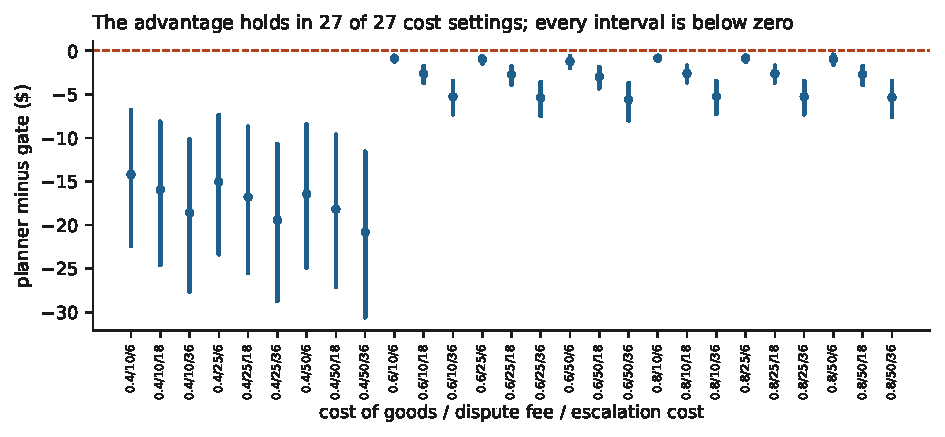
\includegraphics[width=\columnwidth]{../figures/fig2_costs.pdf}
\caption{The paired difference at each of \costSettings{} settings of cost of
goods, dispute fee and escalation cost.}
\label{fig:costs}
\end{figure}

The planner's advantage comes from finding escalation over-priced, so the
obvious objection is that it is an artefact of the benchmark's stipulated costs.
We swept all three over \costSettings{} combinations, rebuilding the corpus and
refitting at each. The planner is better in \costPlannerBetter{} of
\costSettings, and every interval lies below zero
(Figure~\ref{fig:costs}). The mechanism is not that escalation happens to be
expensive at one setting; it is that a fixed rule cannot notice when it is.

\subsection{Does the fitted belief transfer?}

\begin{table}[t]
\centering
\caption{The prior fitted on the public split, applied to a corpus regenerated
from a different seed.}
\label{tab:transfer}
\footnotesize\setlength{\tabcolsep}{2pt}
\begin{tabular}{llrrr}
\toprule
split & prior & gate (\$) & planner (\$) & difference (\$) \\
\midrule
public & fitted on public & 31.37 & 28.63 & -2.74 [-3.82, -1.78] \\
public & fitted on this split & 31.37 & 28.63 & -2.74 [-3.82, -1.78] \\
public & deliberately wrong & 31.37 & 153.04 & 121.67 [81.57, 169.28] \\
hidden & fitted on public & 35.22 & 32.55 & -2.67 [-3.67, -1.75] \\
hidden & fitted on this split & 35.22 & 32.55 & -2.67 [-3.67, -1.75] \\
hidden & deliberately wrong & 35.22 & 201.22 & 166.00 [112.18, 224.48] \\
\bottomrule
\end{tabular}
\end{table}

Fitting on the public split and evaluating on the regenerated one reduces the
mean gap by \$\transferReduction, statistically indistinguishable from the
public-split result.
A deliberately wrong prior, one that says captures resolve early and nearly
always settle, raises the planner's mean gap to \$\wrongPrior. The fit is doing
work and it is not memorising the draw.

\subsection{Shields, and what they are for}
\label{sec:shield}

\begin{table}[t]
\centering
\caption{The shield as a wrapper around policies that do not maximise expected
value, under two criteria.}
\label{tab:shield}
\footnotesize\setlength{\tabcolsep}{3pt}
\begin{tabular}{llrrrr}
\toprule
policy & shield & exact (\%) & mean gap (\$) & paired (\$) & pre-det.\ (\%) \\
\midrule
optimistic & none & 65.7 & 163.61 & 253.53 & 66.0 \\
 & expected & 65.7 & 163.61 & 253.53 & 66.0 \\
 & downside & 32.1 & 244.29 & 192.20 & 7.0 \\
\addlinespace
majority & none & 33.5 & 229.06 & 171.02 & 0.0 \\
 & expected & 33.5 & 226.85 & 167.84 & 0.0 \\
 & downside & 29.9 & 243.53 & 181.46 & 0.0 \\
\addlinespace
react & none & 54.0 & 128.19 & 116.97 & 0.0 \\
 & expected & 54.0 & 128.19 & 116.97 & 0.0 \\
 & downside & 51.8 & 132.68 & 116.97 & 0.0 \\
\addlinespace
eager & none & 14.0 & 298.84 & 226.73 & 0.0 \\
 & expected & 14.0 & 298.84 & 226.73 & 0.0 \\
 & downside & 14.0 & 298.84 & 226.73 & 0.0 \\
\addlinespace
\bottomrule
\end{tabular}
\end{table}

\begin{figure}[t]
\centering
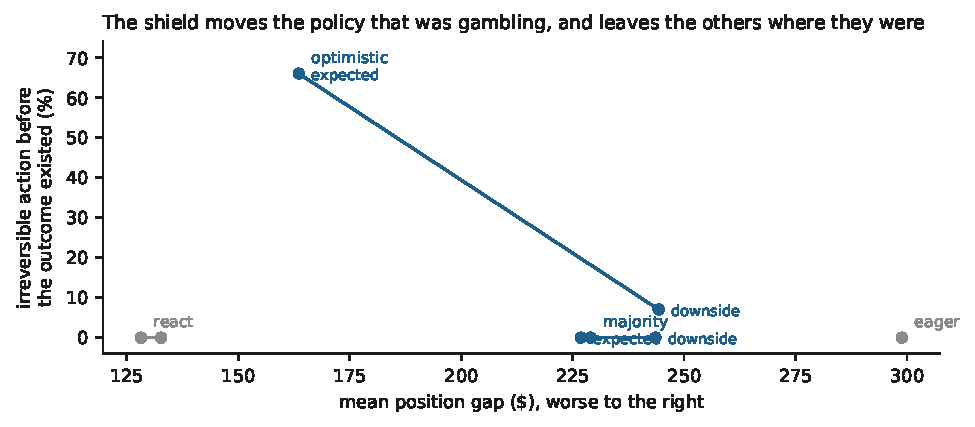
\includegraphics[width=\columnwidth]{../figures/fig3_shield.pdf}
\caption{Each policy under no shield, an expected-value shield, and a downside
shield.}
\label{fig:shield}
\end{figure}

Table~\ref{tab:shield} wraps the shield around four policies. The
expected-value criterion blocks almost nothing, and the reason is worth stating
plainly: goods cost sixty per cent of the order and captures settle
\settleMarginal{} of the time, so shipping without checking has positive
expected value. A criterion built on the mean cannot object to a bet that pays.

The downside criterion objects, on the grounds that the branch it cannot rule
out loses the goods outright. On the ship-on-first-sign policy it cuts
pre-determination irreversible actions from \optPrem\%\ to \optShieldPrem\%\ and
paired loss from \$\optPaired{} to \$\optShieldPaired, while raising the mean gap
from \$\optGap{} to \$\optShieldGap. It buys safety with expected value.

When the shield objects it asks the agent to probe rather than forbidding it to
act. A veto turns a policy that gambles into one that never moves, which we
measured before adopting the redirect and do not recommend.

The two criteria disagree because the benchmark's paired scoring and its natural
outcome distribution disagree. Twin pairs balance settle and fail by
construction, so paired loss prices a gamble at even odds; the corpus as drawn
settles \settleMarginal{} of the time. Both numbers are correct and they answer
different questions. An operator who believes their deployment resembles the
corpus should prefer the expected-value criterion; one who cannot afford the bad
branch on any individual order should prefer the other. This paper does not
claim to settle which, and reports both.

\subsection{Reliability under repetition}

Every task is run under \nSeeds{} fault schedules, and a policy that is right
on some of them and wrong on others is not a policy anyone can deploy. The
planner is exactly right under all \nSeeds{} seeds on \planPassK\%\ of tasks
against the gate's \gatePassK\%. The ReAct loop, which is right \emph{once} on
more than half of tasks, holds up under repetition on \reactPassK\%.

The planner and the gate lose almost nothing to repetition because both decide
from the authoritative channel, which no delivery fault touches. Which schedule
a task draws changes what the replicas say and not what the probe says, so it
changes nothing either policy depends on. That property belongs to the gate's
design and this paper inherits it rather than contributing it.

\section{Discussion}

\textbf{A fixed rule cannot notice what is at stake.} The gate escalates every
unresolved case for the same fee whether the order is worth twenty-five dollars
or three thousand. That is not a bug in the gate; it is what a rule is. The
margin recovered here is the value of making the same decision as a function of
the order rather than as a constant, and the cost sweep is the evidence that the
mechanism is the function and not the particular constants.

\textbf{The useful part of the planner is small.} Two of four components are
inert, and the two that work are a conditional probability and a comparison of
four expressions. This is not a sophisticated planner and it does not need to
be: the decision it improves on is a single choice at a single instant, and most
of the episode is spent doing what the gate already did well.

\textbf{Safety mechanisms need a risk criterion, not a value one.} The clearest
result here is negative. An expected-value shield is inert against a policy that
ships without checking, because at the corpus's settle rate that policy is
making money on average. Only a criterion that asks what happens in the branch
the agent cannot rule out objects. Shields in the literature are typically
rule-based~\cite{shieldagent}, which sidesteps this entirely; a value-based
shield has to choose a functional of the outcome distribution, and the mean is
the wrong one.

\section{Limitations}

\textbf{The margin over the strongest baseline is small.} \$\vsGateReduction{}
per episode is a real difference with an interval that excludes zero, and it is
not
a large one. The honest summary is that a careful planner recovers a modest
amount from a good procedure, and a great deal from a mediocre one.

\textbf{Half the method is inert.} Two of the four components contribute
nothing measurable. They are reported rather than removed because the reason the
shield is inert is itself a result, but a reader should understand the working
parts as the decision rule and the conditional prior.

\textbf{The margin depends on how an escalation is modelled, not only on what
it costs.} Of the \$\vsGateReduction{} total, \$\escalatingContribution{} comes
from
the \texttt{\escalatingArchetype} archetype, where the gate escalates.
FinalityBench models an escalated case as an analyst who completes the
disposition of money already held and does not initiate new money movement.
Under that model escalation cannot rescue a capture that never settles, so
declining to escalate is nearly free. The cost sweep varies the price of
escalation and not its effect, and the second assumption carries more weight,
so we measured it.

\begin{table}[t] \centering \caption{Mean position gap over the finality gate
as the analyst becomes more capable. \texttt{retry} is the probability that an
escalated case whose capture could have been re-attempted successfully is
rescued. The first row is FinalityBench's own analyst.} \label{tab:escalation}
\footnotesize \begin{tabular}{rrrr}
\toprule
retry & planner & gate & gap \\
\midrule
0.0 & \$28.63 & \$31.37 & \$2.74 \\
0.2 & \$28.63 & \$31.00 & \$2.37 \\
0.4 & \$28.63 & \$30.63 & \$2.00 \\
0.6 & \$28.63 & \$30.26 & \$1.63 \\
0.8 & \$28.63 & \$29.90 & \$1.26 \\
1.0 & \$28.63 & \$29.53 & \$0.89 \\
\bottomrule
\end{tabular}
 \end{table}

Every graded episode is re-scored under an analyst of a stated capability,
computed after the fact from the log and the case's own retry flag, so the
benchmark is not modified and its published numbers are the \texttt{retry}
$=0$ row. Table~\ref{tab:escalation} gives the sweep. The gap falls from
\$\escBaselineGap{} to \$\escFullGap{} as the analyst goes from never
re-attempting to always succeeding where a retry could work, which is
\escShrink\% of the margin. It does not change sign at any capability.

So both halves of the concern are answered and only one of them favours us.
The margin really is mostly an artifact of what escalation is worth: two
thirds of it disappears against a maximally capable analyst. The ordering is
not: even that analyst leaves the decision rule ahead, because only
\escRescuable{} of the gate's \escEscalations{} escalations
(\escRescuablePct\%) are on cases a retry could have rescued at all. An
analyst with capabilities this model does not represent, one who contacts the
customer or extends the ship-by date, is outside what we can say.

\textbf{The cost settings are correlated.} The \costSettings{} combinations
reuse one corpus generator, one task draw and one set of fault seeds. They show
that the sign of the effect is stable across the region of cost space examined.
They are not \costSettings{} independent confirmations.

\textbf{One environment.} Everything is measured inside FinalityBench, whose
economics are stipulated. The cost sweep addresses whether the conclusion
depends on the particular numbers; it does not address whether the four-term
model of a merchant's position is the right model.

\textbf{No language model.} The planner is a deterministic procedure, and the
shield was tested only around other deterministic procedures. Whether a shield
helps a stochastic agent, which is the case that motivates shields in the
literature, is untested here.

\textbf{The value-of-information rule is not the one that was planned.} This
work was scoped to derive the worth of an observation from causal attribution
over the same benchmark's traces~\cite{causalloss}, which identifies which
messages actually changed an outcome. What is implemented instead estimates the
probability that anything has resolved since the last look, which is cruder and,
on this environment, worth nothing. Whether the causal version would do better
is untested, and the negative result reported here is about the cruder rule.

\textbf{The prior needs a corpus.} Fitting the belief requires a labelled split
with observed resolution times. A deployment without that history would need
either an uninformative prior, which the transfer experiment suggests is
expensive, or an online estimate.

\section{Conclusion}

Escalating to a human is the safe answer to uncertain finality and it is not the
best one, because it costs the same whatever is at stake. Pricing the
alternatives instead recovers \$\vsGateReduction{} per episode against the
strongest policy the benchmark ships, holds across every cost setting we tried,
and transfers to a corpus the belief was not fitted to. What does the pricing is
a deterministic rule evaluated once, at the deadline: a conditional settle
probability and a comparison of four closed-form expressions, with no search
over action sequences and no language model anywhere in the loop. The safety shield that
accompanied the planner turned out to be inert inside it, and chasing that
produced the more useful observation: at these economics an expected-value
shield cannot refuse a profitable gamble, and only a criterion that looks at the
branch it cannot rule out will.

\section*{Artifact availability}

Code, the fitted priors and every result file are at
\url{https://github.com/abhisheksharma2411/finality-aware-planning}, MIT
licensed, at release \texttt{v1.0.2}, which is the revision this paper was
built from. The release is archived at \textsc{doi}
\mbox{10.5281/zenodo.24406794}, which resolves to the current version. It
consumes FinalityBench~\cite{finalitybench} at revision \texttt{0b01661},
which \texttt{make setup} fetches, rather than
reimplementing it; that revision carries a module this paper imports which
P1's tagged releases do not.
\texttt{make reproduce} runs the suite end to end from a clean tree.

\begin{thebibliography}{10}

\bibitem{finalitybench}
A.~Sharma, ``FinalityBench: An effect-level benchmark for agent decisions under
delayed and conflicting financial finality,'' arXiv:2609.04706, 2026,
\textsc{doi}: \mbox{10.5281/zenodo.22262591}.

\bibitem{causalloss}
A.~Sharma, ``CausalLoss-Fin: Attributing financial-agent loss to decisions and
infrastructure faults,'' arXiv:2609.25960, 2026,
\textsc{doi}: \mbox{10.5281/zenodo.22893020}.

\bibitem{actorescalate}
M.~DosSantos DiSorbo and H.~Ju, ``Act or escalate? Evaluating escalation
behavior in automation with language models,'' arXiv:2604.08588, Mar. 2026.

\bibitem{abstention}
H.~Luo, B.~Wen, and L.~L.~Wang, ``Agentic abstention: Do agents know when to
stop instead of act?,'' arXiv:2606.28733, Jun. 2026.

\bibitem{shieldagent}
Z.~Chen, M.~Kang, and B.~Li, ``ShieldAgent: Shielding agents via verifiable
safety policy reasoning,'' arXiv:2503.22738, Mar. 2025.

\bibitem{voimcp}
Z.~Laouar, Q.~H.~Ho, and Z.~Sunberg, ``Leveraging the value of information in
POMDP planning,'' in \emph{Proc. ICAPS}, vol.~36, no.~1, 2026, pp. 152--160,
\textsc{doi}: \mbox{10.1609/icaps.v36i1.42824}.

\bibitem{coststopping}
Y.~Feng, Y.~Zhang, Y.~Cheng, and W.~Qi, ``Scores are not decisions: Cost-aware
stopping for tool acquisition in LLM agents,'' arXiv:2607.27083, Jul. 2026.

\bibitem{verifiedtools}
I.~K.~Mansoor, A.~Phadke, and P.~Rana, ``Verified tool calls improve LLM agent
reliability under non-atomic failures,'' arXiv:2608.02645, Jul. 2026.

\bibitem{trustbound}
S.~Nandi, A.~Bose, A.~Bose, and S.~Bakshi, ``TrustBound: Mechanized
completeness for payment epochs initiated by AI agents,'' arXiv:2611.19551,
Nov. 2026.

\bibitem{revisable}
Z.~Zhai, M.~Li, and X.~Wang, ``Revisable by design: A theory of streaming LLM
agent execution,'' arXiv:2604.23283, Apr. 2026.

\end{thebibliography}

\end{document}
